%%%%%%%%%%%%%%%%%%%%%%%%%%%%%%%%%%%%%%%%%%%%%%%%%%%%%%%
% LaTeX template ~ 'tau-book.tex'
%
% Description: Tau-book is a LaTeX template that offers
% a clean and professional design for lab reports or
% academic papers. The clarity of the code structure
% makes it easy to understand and modify for your needs.
% This template uses an easy-to-read font and high
% quality equations with "stix2".
%
% Version 2.0 (03/03/2024)
%
% Author:
% Guillermo Jimenez (memo.notess1@gmail.com)
%
% License:
% Creative Commons CC BY 4.0
%%%%%%%%%%%%%%%%%%%%%%%%%%%%%%%%%%%%%%%%%%%%%%%%%%%%%%%
% You may modify 'tau-book.cls' file according to your
% needs and preferences. This LaTeX class file defines
% the document layout, formatting, and behavior.
%%%%%%%%%%%%%%%%%%%%%%%%%%%%%%%%%%%%%%%%%%%%%%%%%%%%%%%
%   BIBLIOGRAPHY WITH BIBLATEX IN EXTERNAL EDITORS:
% If the bibliography does not show up, run the 'tau.cls'
% with biber in MikTeX console two times and re(run)
% 'tau-book.tex'. If the problem continues, try
% running 'tau.bib' with biber and re(run) 'tau-book.tex'.
%%%%%%%%%%%%%%%%%%%%%%%%%%%%%%%%%%%%%%%%%%%%%%%%%%%%%%%
%                       WARNING:
% It is important to proceed with caution and ensure
% that any modifications made are compatible with LaTeX
% syntax and conventions to avoid errors or unexpected
% behavior in the document compilation process.
%%%%%%%%%%%%%%%%%%%%%%%%%%%%%%%%%%%%%%%%%%%%%%%%%%%%%%%

\documentclass[10pt,a4paper,twoside]{main}
\usepackage[english]{babel}
\usepackage{kappa}

%------------------------------------------------------
% Title
%------------------------------------------------------

\title{Development of an IoT-Based Virtual Fencing System with Advanced Monitoring and Animal Tracking Capabilities}

%------------------------------------------------------
% Authors, affiliations & professor
%------------------------------------------------------

\author[a,1]{Simanga H. Khoza}
% \author[b,2]{Author 2}
% \author[b,c,3]{Author 3}

%------------------------------------------------------

\affil[a]{Department of Computer Systems}
% \affil[b]{Department of Biology}
% \affil[c]{University of Alpha}

\professor{Student Number: 214651459}

%------------------------------------------------------
% Footpage notes
%------------------------------------------------------

\institution{College name}
\ftitle{Writing in \LaTeX}
\theday{March 3, 2024} % \today
\etal{et al.}
\course{\LaTeX\ Template}

%------------------------------------------------------
% Abstract
%------------------------------------------------------

\theabstract{
    The demand for beef is on the rise as the global population grows, despite the
    availability of alternative protein sources. In order to meet this increasing
    demand, it is essential to enhance the efficiency of beef production. This
    paper proposes for a virtual fencing system that utilizes
    IoT technology to assist farmers in efficiently managing and monitoring their
    cattle. While other industries have already benefited from data monitoring and
    tracking, the agricultural sector has been slower to adopt these technologies.
    By implementing live monitoring of livestock, farmers can reduce labor costs and
    improve overall farm management, leading to more effective yearly planning for
    busy farms.
}

%------------------------------------------------------

\keywords{\LaTeX\ class, template, laboratory report, college}

%------------------------------------------------------

\begin{document}

    \maketitle
    \abscontent
    % \tableofcontents  % Uncomment to activate the table of contents
    \thispagestyle{firststyle}

%------------------------------------------------------
% The document begins
%------------------------------------------------------

\section{Introduction}

    \taustart{I}n the field of academic and professional document creation, having a well-designed template can greatly streamline the writing process and ensure a good final product. Introducing the ``tau-book.cls'' class, a clean and minimalist template designed for a wide range of document types, mainly academic papers and lab reports.

    Due to its clean and structured code, users can easily customize this class to their specific needs and preferences. In addition, this template uses an easy-to-read and high-quality font in equations with ``stix2''. Notable features include custom colors and settings for including notes, information and code from Matlab, C, C++ and \TeX.

    \subsection{Explanation}

        Throughout this guide, we will teach how to effectively use the ``tau-book'' template to ensure that users can take advantage of its potential. We will provide detailed instructions on customization options, allowing users to personalize the template to their specific needs and preferences.

    \subsection{Specs}

        The main document ``tau-book.tex'' is designed for \textit{A4paper}, \textit{letterpaper} or \textit{legalpaper}. Using the geometry package, which specifies margins and layout dimensions, the template ensures optimal readability and aesthetic appeal, with carefully selected settings.

\section{Title and abstract}

    The \textit{maketitle} command generates the title and author information section, including the title, author name, professor/supervisor name, and affiliations.

    Then, the abstract and keywords are defined using the \textit{theabstract} and \textit{keywords} commands respectively. The abstract provides a concise summary of the article's content, while the keywords help in indexing and searching the article.

    The ``tau-book.cls'' document class provides a convenient way to automatically adjust the language-specific headings like ``Abstract'' and ``Resumen'' based on the document's language settings.

    This ensures seamless integration for documents written in both English and Spanish, allowing users to focus on content creation without worrying about manual adjustments for multilingual support.

    In the code \ref{lst:listing-tex}, we show the part where you can make the manual modification in case you choose another language not defined by the class.

    \lstinputlisting[caption=Abstract language code, label={lst:listing-tex}, language=Tex]{example.tex}

    You will find the code in the ``tau-book.cls'' file in the ``textit{abstract preferences}'' section (line 137-143).

\section{Aesthetics}

    \subsection{Tau start}

        In this \LaTeX\ document, we've included the \textit{taustart} command, which provides a personalized lettrine for the beginning of a paragraph. This command is defined with two parameters: the dropcap font size and the content of the lettrine itself. It is utilized within the Introduction section to enhance the visual appeal and style of the article.

        This attention to detail adds a touch of elegance and professionalism to the document, ensuring a captivating reading experience.

    \subsection{Stix2 font package}

        This \LaTeX\ template uses the stix2 font package to maintain a clean, elegant and professional look. The stix2 font provides excellent legibility. By incorporating this font package, the document maintains a consistent and clean aesthetic throughout, especially when writing equations.

    \subsection{Table of contents}

        The Tau-book class provides a table of contents that presents a hierarchical structure that organizes the contents of the document. It begins with the main sections, followed by subsections that expand on those topics and, in turn, the subsubsections provide additional details. Each level of the table of contents provides a preview of the content and its location in the document, making it easier to navigate and understand the document.

    \subsection{Header and footer}

        Headers and footers are designed to provide relevant and contextual information about the paper. The header shows the title of the paper, while the footer contains details such as the institution, date, paper title and authors' surnames. This arrangement ensures that readers have access to key information at all times, making the document easier to understand and reference.

    \subsection{Caption}

        \subsubsection{Figures}

            The provided \textit{captionsetup} command customizes the appearance of captions for figures in \LaTeX\ documents. It adjusts various aspects of the caption style such as format, label separator, font style and size, justification, and label font size. This setup ensures that figure captions are presented in a consistent and visually pleasing manner throughout the document. For example, in Fig. \ref{fig:enter-label}, the caption will appear with the specified formatting.

            \begin{figure}[H]
                \centering
                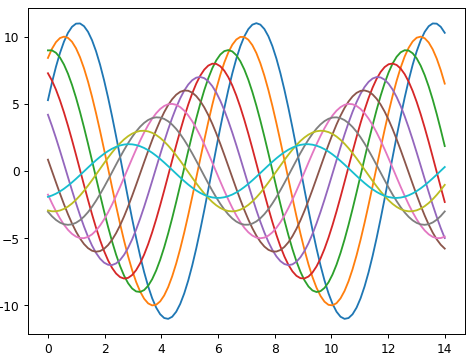
\includegraphics[width=\columnwidth]{Figures/Lines.png}
                \caption{Example of a figure}
                \label{fig:enter-label}
            \end{figure}

        \subsubsection{Tables}

            The \textit{captionsetup} command customizes the appearance of the captions in the document. The default table caption will display the caption below, however, there is an alternative to display the caption above the table. To do this, open the ``tau-book.cls'' class document and find the ``table caption style'' section then, change the position to above. For example, in Table \ref{tab:example}, the caption will appear with the specified formatting.

            \begin{table}[H]
                \centering
                \begin{tabular}{cc}
                    \textbf{Column 1} & \textbf{Column 2} \\
                    \midrule
                    Data 1 & Data 2 \\
                    Data 3 & Data 4 \\
                    \bottomrule
                \end{tabular}
                \caption{Small table example}
                \label{tab:example}
            \end{table}

            In the "tau-book.cls", you could also set the caption above the table, to customize the document as you prefer; mentioned before.

    \subsection{Equation}

        The ``amsmath'' package, short for ``American Mathematical Society mathematics'', is an essential tool in \LaTeX\ for typesetting mathematical equations with precision and clarity. It extends LaTeX's native math typesetting capabilities by providing a comprehensive suite of environments and commands for mathematical notation.

        \begin{equation}
            \int_{0}^{\pi} \frac{x^2}{\sqrt{1 + x^4}} \sin(x) \, dx
        \end{equation}

    \begin{info}
        The ``amssymb'' package was not necessary to include, because the stix2 font incorporates mathematical symbols for writing quality equations. In case you choose another font, include the package to avoid compilation problems.
    \end{info}

    \section{Environment}

        The "tau book" class includes custom environments designed to enhance the presentation of information within documents. Among these custom environments are ``info'' and ``note'', which are characterized by their minimalist and aesthetic design. However, users also have the option to include other custom environments such as ``info2'', ``link'' and ``warn'' for different purposes.

        The ``info'' and ``note'' environments are particularly recommended for their clean and visually appealing appearance. The ``info'' environment provides a structured format for presenting informative content, while the ``note'' environment highlights important notes or remarks. Both environments feature a consistent design with a blue background and bolded titles for clarity.

        For instance, the ``note'' environment is defined with specific styling attributes, including a blue background color, bolded title, and italicized font for the content. Additionally, the frame title is aligned to the left for improved readability. These attributes contribute to a cohesive and professional presentation of information within documents.  Users can take advantage of these customized environments to organize and convey information in an effective and visually appealing manner.

        You may also costumize these environments located at the end of ``kappa.sty'' personalized package (line 241-295).

        \begin{note}
            These environments, such as the summary section, modify the title according to the selected language (english or spanish).
        \end{note}

\section{Coding}

    The ``kappa'' package includes the "listings" package, which offers versatile and customizable features for typesetting code snippets in \LaTeX\ documents. Specifically for C, C++, \TeX\ and MATLAB codes. The ``listings'' package allows users to present code blocks with syntax highlighting, line numbering, and various formatting options to enhance readability and comprehension.

    For C and C++ codes, the ``listings'' package recognizes the syntax of these programming languages and highlights keywords, comments, and string literals accordingly. This makes it easier for readers to distinguish between different elements of the code and understand its structure. Additionally, line numbering can be enabled to provide reference points within the code snippet.

    \lstinputlisting[caption=Example of C code, label={lst:listing-c}, language=C]{example.c}

    Similarly, for MATLAB codes, the ``listings'' package offers syntax highlighting and line numbering, to the MATLAB language syntax. This is particularly useful for including MATLAB scripts.

    \lstinputlisting[caption=Example of matlab code, label={lst:listing-Mat}, language=Matlab]{example.m}

\section{References}

    In the ``tau-book'' class, the default formatting for references follows the IEEE style. This style is commonly used for technical documents, research papers, and scholarly articles in engineering and computer science fields. It provides a structured and standardized format for citing sources, making it easy to locate and reference relevant literature \cite{einstein}.

    However, the ``tau-book'' class \cite{dirac} also offers the flexibility to customize the formatting of references through its internal settings. By modifying the settings in the ``tau-book.cls'' file, users can adjust the citation and bibliography styles to suit their specific preferences to the requirements of different publication guidelines.

    At the end of the document, you will find an example of the default reference formatting in the ``tau-book'' class. Additionally, the ``tau.bib'' file provided can serve as an example for future citations. This BibTeX file contains sample bibliographic entries that demonstrate how to format references according to the IEEE style.

\section{Updates}

    \subsection{Tau-book class - Version 2}

        In version 2 of ``tau-book.cls'' new improvements and general fixes have been introduced. One of these major improvements is the table of contents, where it has been designed to have a style compatible with the template providing a more professional appearance and adapted to the user's needs.

        The subtitle formats have been modified, allowing for a more esthetically presentation of the document content. Finally, general corrections have been made to the document for the overall quality of the document.

%------------------------------------------------------

\printbibliography

%------------------------------------------------------

\end{document}
